\documentclass[12pt]{article}
\usepackage[parfill]{parskip}
%Mathematical TeX packages from the AMS
\usepackage{amssymb,amsmath,amsthm} 
%geometry (sets margin) 
\usepackage[margin=1.25in]{geometry}	
\usepackage{enumerate}					
\usepackage{graphicx}
\usepackage{amsfonts}
\usepackage{hyperref}
\usepackage{subfigure}

\theoremstyle{plain}% default
\newtheorem{thm}{Theorem}[section]
\newtheorem{lem}[thm]{Lemma}
\newtheorem{prop}[thm]{Proposition}

\theoremstyle{definition}
\newtheorem{defn}{Definition}[section]
\newtheorem{conj}{Conjecture}[section]
\newtheorem{exmp}{Example}[section]

\theoremstyle{remark}
\newtheorem*{rem}{Remark}
\newtheorem*{note}{Note}
\newtheorem{case}{Case}

\begingroup
    \makeatletter
    \@for\theoremstyle:=definition,remark,plain\do{%
        \expandafter\g@addto@macro\csname th@\theoremstyle\endcsname{%
            \addtolength\thm@preskip\parskip
            }%
        }
\endgroup
%=============================================================
%Fancy-header package to modify header/page numbering 
%
\usepackage{fancyhdr}
\pagestyle{fancy}
\lhead{Wesley Chen, Brandon Sim}
\chead{} 
\rhead{\thepage} 
\lfoot{\small Applied Math 120} 
\cfoot{} 
\rfoot{\footnotesize Automating Brain Tumor Detection in MRI Images} 
\renewcommand{\headrulewidth}{.3pt} 
\renewcommand{\footrulewidth}{.3pt}
\setlength\voffset{-0.25in}
\setlength\textheight{648pt}

%=============================================================

\begin{document}

\title{Automating Brain Tumor Detection in MRI Images}
\author{Wesley Chen, Brandon Sim}

\maketitle
\tableofcontents
\newpage

\section{Introduction and Motivation}

Magnetic resonance imaging, or MRI, is one of the most accurate and available types of medical imaging that is used to detect diseases throughout the body, ranging from severe bleeding to cancerous growths (SOURCE A).  The prevalence of MRI scans for diagnosis in the medical field is well represented by the sheer number of expensive yet critical MRI equipment - there are over 10,000 MRI machines in just the United States alone (SOURCE B).  When a doctor administers an MRI scan. the machine stores many 2D slices of the brain. These scans are also taken from various axials. From this collection of slices, the doctor must look through each frame for possible irregularities that could confirm the existence of a tumor.  The person reading the MRI image must flip through each of the hundreds of frames systematically - there is no shortcut to knowing about where a tumor could be.  Often times, the doctor must look at the same images multiple times even if her or she does not see a tumor just to make sure a small tumor (which could be as large as just spanning 3 frames and only tens of pixels) was not missed.  The requirement of such a methodical but tedious search inspired us to develop approaches to automate the reading of a set of MRI images. For the scope of this project, we limited our dataset to MRI images of the brain. We explored traditional image processing techniques as well as developed our own more specialized technique to identify possible tumor candidates from a given 2D image (one slice of the brain). We then extended this search to an entire stack of images representing the full 3D brain. Although we recognize that our algorithm will probably not fully replace a doctor's screening of MRIs, for liability and accuracy concerns, we do hope that it will both serve as a valuable backup ``safety net'' for the doctor, as well as be able to suggest likely tumor candidates that the doctor can focus special attention on.

\section{Methodology}

We were given a complete data set of a MRI brain scan for one patient with a relatively small tumor, courtesy of Dr. Steven Shufflebeam of Massachusetts General Hospital.  Using a small tumor as our test case, we believe that larger tumors will only be more obvious to identify.
We tried two independent approaches to ideentifying a positive tumor case out of a given 2D frame: the first was using watershed segmentation to filter various foreground objects – hoping to identify the tumor as one of the fewer remaining objects.  A brain tumor usually appears as a denser, white area which should be filtered out by the segmentation algorithm.  Because this algorithm relies on 3D detail which our 2D scan did not have, we tried a simpler, more elegant method, 2D-limited strategy.

The second method we used was based on a symmetry analysis algorithm.  A tumor should be recognized as a closed object in our image.  We could identify this closed region from an edge detection step.  Then, we wanted to use the natural symmetry of the brain to detect the tumor.  A tumor would be an irregular growth and would not have a symmetric counterpart.

If either method worked, we would save the 3D location (using the frame number).  We woudl then check which tumor candidates came up consistent across several consecutive frames - and these would be identified by our final program output.

\subsection{Watershed Segmentation}

The goal of the watershed segmentation method is to map the image to a topological equivalent, and ``flood out"� various ``basins''to represent different levels of foreground.  The first step would be to convert to grayscale.  The intensity of the grayscale code would be mapped to relative height.  Conceptually, once this grayscale mapping is complete, the “whitest” pixels would represent areas of maximum height (or intensity or density in the case of an MRI image).  Using a gradient magnitude should result in proper segmentation.  However, due to small differences in gradient, this results in an overly segmented product (see results section below).

To eliminate such detail, a set of image erosion and dilations must be conducted to eliminate some foreground detail.  The foreground is selected through a morphological structuring element provided by the \verb|strel()| function of \textsc{Matlab}'s image processing toolkit.  We chose to use ``disk'' shaped elements as the round object best represents the structures we would find in the brain.  We then calibrated the size of this element and this is where we controlled the level of segmentation.  This element is used by the image manipulation functions below.

After this element is created, we used other Matlab image processing functions (namely \verb|imerode()| and \verb|imdilate()|) to help remove foreground detail and provide a map of topological height “most prominent foreground areas. \verb|Imerode()| and \verb|imdilate()| are complimentary functions that look at every subset of the disk shaped element within the full image matrix to find areas with very similarly colored pixels - combining them into a gradual gradient.  In other words, it dilates the detail of the foreground to produce more uniform areas that won't over-segment when running a watershed algorithm. 

After the establishment of the foreground markers, the markers were superimposed over the original image.  Another sequence of erosion-dilation was applied to help smooth out the foreground markers superimposed onto the original image.  Then, a grayscale thresholding function was run to select the background areas.  Anything darker than a certain threshold would be marked as ``background''�. Then, the \verb|watershed()| function was called to create ridges (the valleys of the basin area - also our background).  This background marker image was then superimposed onto the image with the foreground marker to create the fully marked image.  In our MRI case, because the background is uniformly black, this step was not necessary but was kept in our program for comprehensiveness (will still work on any image).

Finally, we visualized the result by using a colored watershed visualization which filled each object with a different color.  This color map was then superimposed with a 50\% transparency over our original image.  Then, each color would be a different component to identify as a possible tumor candidate.
	
\subsection{Symmetry Analysis}

The second approach we used was a more unique one designed to take advantage of the highly symmetric nature of the brain. Our hypothesis was that, while many features of the brain are symmetric in the brain, tumors would most likely not be symmetric. This reasoning led us to create the following algorithm:

\begin{enumerate}
\item We first detect the axis of symmetry of the brain with respect to the image by finding the ellipse that has the same normalized second central moment as the region in question and calculating the orientation of its semimajor axis with respect to the x-axis of the image.
\item We detect the edges using the Canny edge detection operator, which we choose over other edge detection algorithms such as the Sobel operator because it uses hysteresis thresholding rather than fixed thresholding. Although it does require more computational time to run, it results in an algorithm that is more robust to noise and avoids multiple edge lines.
\item We detect all closed edges; that is, edges which form a curve that completely enclose some area.
\item We reflect each closed object detected in the image across the axis of symmetry, and calculate the overlapping number of pixels for each set of objects, pairwise. Those pairs of closed objects with the lowest overlapping area are the areas with highest likelihood of being tumors.
\item Finally, as an additional checking measure, we generate ellipses with the same normalized second central moment as each of the Canny-filtered closed regions and find their centroids. This step will be the basis of the second part of our symmetry analysis and will be discussed more in detail later.
\end{enumerate}


Mention smoothing, thresholds

DID YOU WANT TO TALK ABOUT RANKING THE AREAS?

The dude’s edge list library – CITE BELOW

\subsection{Expansion to Full Image Set}

Region functions like the ellipse things

CENTROID,

TALK ABOUT THE MULTIPLE SLICES HERE

\section{Results}

For both cases, we started with the 2D MRI snapshot below that we selected from the stack as it clearly shows the tumor - the white area located in the bottom left quandrant.

\begin{figure}[!h]
	\centering
		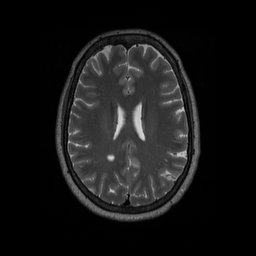
\includegraphics{original.jpg}
	\caption{Original 2D Tumor Image}
\end{figure}

\subsection{Watershed Segmentation}

Because the watershed segmentation algorithm is designed for more complex (3D), we will also show the output for a given colored image, this lily pad landscape in addition to the MRI image.

\begin{figure}[!h]
	\centering
		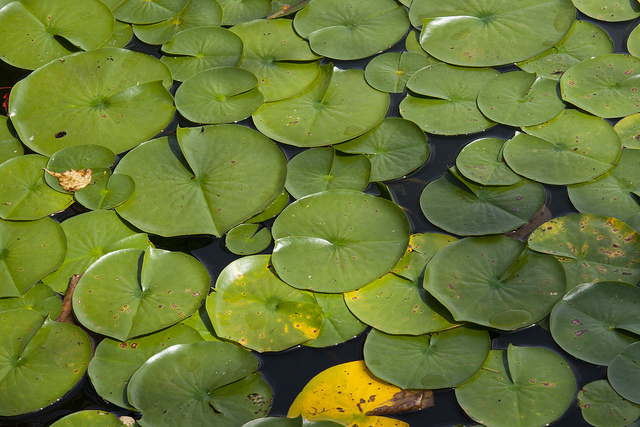
\includegraphics[width=0.9\textwidth]{lilypad.jpg}
	\caption{Original Lilypad Landscape}
\end{figure}

The end output, the colored watershed visualization after image processing superimposed onto the original image is shown below.

\begin{figure}[!h]
	\centering
		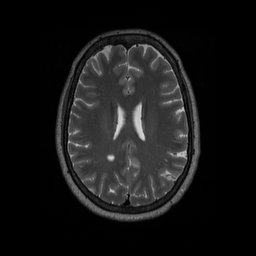
\includegraphics{original.jpg}
	\caption{Colored Watershed Segmentation of Processed MRi image.  Notice that the tumor region is successfully identified as a unique area.  however, due to the 2D subject of an MRI image, the algorithm overcomplicates the foreground and identifies various other regions as false positives as well (see Discussion)}
\end{figure}

\begin{figure}[!h]
	\centering
		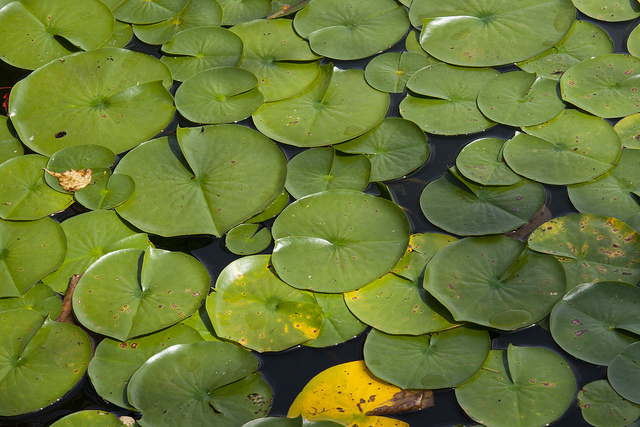
\includegraphics[width=0.9\textwidth]{lilypad.jpg}
	\caption{Colored Watershed Segmentation of Processed Lilypad Landscape.  With this 3D example, one can see that the image algorithm successfully reduces the 3D subject of the image to unique regions and represents them with different colors}
\end{figure}

For results of each individual step, please refer to Appendix A.

\subsection{Symmetry Analysis}

\subsection{Expansion to Full Image Set}

\section{Discussion}

The results from the image processing methods show much cleaner results for the symmetry analysis approach.  This is most likely because the image processing algorithm assumes 3D level of detail for the image (selecting a foregournd and a background).  When the 2D MRI image does not represent a 3D picture, there is a loss of data that helps the image filters work.  thus we see some random articfacts in the watershed approach.

The symmetry analysis, as a much more simple algorithm, gave us remarkably better results.  We recognize, however, that this algorithm is limited by the symetry.  Therefore, we cannot extend this algorithm to process other parts of the body that are assymetrical, unlike that of the image processing algorithm.

We are also aware that individually, both algorithms need to be semi-calibrated to give us the best output.  When run using auto-thresholding, the watershed segmentation method has a tendency to provide false positives due to the fact that the tumor is not the absolute brightest structure recorded by the MRI.  It would be difficult to “teach” our algorithm to ignore such areas – because sometimes, the tumor could in fact be the brightest area.  However, this problem can be reduced by running the algorithm at various thresholds for the morphological structure element used to simplify the image.  Regardless, providing false positives is more acceptable than a false negative – as a doctor would be able to quickly filter through the highlighted possibilities for tumor candidates.

The edge detection algorithm requires a similar calibration step - setting the hystersis threshold for the Gaussian filter .  The same process to test various thresholds for repeated results would help reduce these errors.  Because of the simplicity of this design, this algorithm seems to be favored with our current results.  One weakness of the symmetry based edge detection is that there may be false negatives (if the tumor is bordering another edge), an error that is less desirable in medical applications.

Because the algorithms are independent in their approaches, successive application of the two would only improve our confidence.  Through such cross-checking, the agreed parts would have the highest probability of being the area of interest.  Combining both methods would increase our detection rate while minimizing false positives.

\section{Conclusion and Further Work}

Our project has demonstrated two possible independent directions to the automation of MRI reading.  The beauty of the symmetry analysis is that it works well for the naturally symmetric brain.  The simpler algorithm gives us much cleaner results that we refined output tumor candidates given the entire stack of MRI images.  Perhaps we could run some similar approach on the watershed segmentation algorithm to help refine its results.  We would also like to aquire more data so as to demonstrate the robustness of our algorithm.  Beacuse our code is extremely modular and has limited magic numbers, we do not anticpate any complications when expanding to a new data set.

We believe that our two algorithms will work well with each other and when coordinated, will provide the best results.  We would like to coordinate the two algorithms.  This could be done by storing the coordinates of each candidate area.  We could then cross check using the MRI images from a different angle.  These steps would conclue our project in a fully-functional, automated MRI interpreter.  Even if it is unable to conclusively diagnosis a tumor, this program could at least reduce the number of frames that a doctor would have to sift through to identify a possible tumor.  And beyond that, we would also be able to output a “best candidate” confirmed by multiple approaches.

We invite you to view all of our code at \url{https://github.com/bksim/images}.
\section{References}
\begin{enumerate}
\item \textsc{MATLAB} - image processing toolbox
\item http://www.mathworks.com/products/image/examples.html?file=/products/demos/shipping/images/ipexwatershed.html\#2
\item SOURCE A http://www.medicinenet.com/mri\_scan/article.htm
\item SOURCE B http://www.magnetic-resonance.org/MagRes\%20Chapters/21\_03.htm
\item SOURCE C http://12000.org/my\_courses/UCI\_COURSES/CREDIT\_COURSES/fall\_2004/EECS\_207A\_UCI\_FALL\_2004\/my\_notes\/nabbasi\_EECS\_207A\_notes.pdf

\end{enumerate}
	
\section{Appendix A: Watershed Segmentation Images}

\begin{figure}[!h]
	\centering
		\mbox{\subfigure[Recall the original image MRI image]{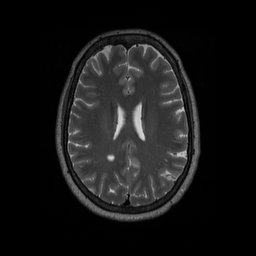
\includegraphics[width=0.45\textwidth]{original.jpg}}\quad
		\subfigure[the original lilypad image]{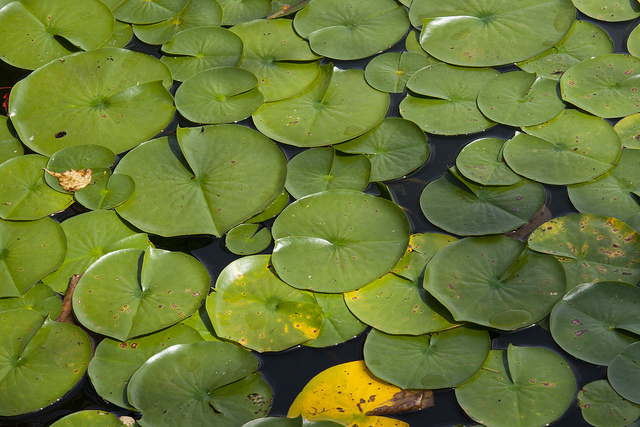
\includegraphics[width=0.45\textwidth]{lilypad.jpg}}}
\end{figure}

\section{Appendix B: Symmetry Analysis Images}

\section{Appendix C: \textsc{MATLAB} code}
\subsection{Watershed Segmentation Code}
Treats the input image across various filters to display the final watershed segmented color overlay.
\subsubsection{filename.m}
\begin{verbatim}
%generalized watershed method starting with colored image

%read image - using lilypad.jpg, a colored, 3D landscape of lilypads
I = imread('lilypad.jpg');

%convert RGB into grayscale
I = rgb2gray(I);

%horizontal edge filter
hy = fspecial('sobel');
%vertical component
hx = hy';

%use image filter, needs "double" input, filter, option
Iy = imfilter(double(I), hy, 'replicate');
Ix = imfilter(double(I), hx, 'replicate');

%calculate gradient
gradmag = sqrt(Ix.^2 + Iy.^2);
figure(1), imshow(gradmag, []), title ('Gradient Magnitude')

%export this figure, need to scale range so coudln't just imwrite
print (1, '-djpeg', 'Gradient_Mag')

%demonstrate oversegmentation of direct watershed of gradient
L = watershed(gradmag);
Lrgb = label2rgb(L);
figure(2), imshow(Lrgb, []), title('Oversegmented Watershed')

%export this figure (couldn't export image due to transparency)
print (2, '-djpeg', 'Overseg_Watershed')

%create disk shaped morphological structuring element of size 6 - picked so
%not to over or under segment, disk shaped as target structure is round
se = strel('disk', 6);

%first method to open: (imopen)
Io = imopen(I, se);
imwrite(Io, 'Open_Disk6.jpg', 'jpg');
%figure, imshow(Io), title('Opening (Io)')

%second method to open: reconstructed (imerode)
Ie = imerode(I, se);
Iobr = imreconstruct(Ie, I);
imwrite(Iobr, 'OpenReconstuct_Disk6.jpg', 'jpg');
%figure, imshow(Iobr), title('Opening-by-reconstruction (Iobr)')

%first method of closing: (imclose)
Ioc = imclose(Io, se);
imwrite(Ioc, 'Close_Disk6.jpg', 'jpg');
%figure, imshow(Ioc), title('Opening-closing (Ioc)')

%second method to close: reconstructed (imdilate)
Iobrd = imdilate(Iobr, se);
Iobrcbr = imreconstruct(imcomplement(Iobrd), imcomplement(Iobr));
Iobrcbr = imcomplement(Iobrcbr);
imwrite(Iobrcbr, 'CloseReconstruct_Disk6.jpg', 'jpg');
%figure, imshow(Iobrcbr), title('Opening-closing by reconstruction (Iobrcbr)')

%use function to store maxima (foreground marker)
fgm = imregionalmax(Iobrcbr);
imwrite(fgm, 'Maxima.jpg', 'jpg');
%figure, imshow(fgm), title('Regional maxima of opening-closing by reconstruction (fgm)')

%copy image and superimpose to form new working image
I2 = I;
I2(fgm) = 255;
imwrite(I2, 'MaximaSuperimposed.jpg', 'jpg');
%figure, imshow(I2), title('Regional maxima superimposed on original image (I2)')

%create a new morphological element to smooth out the foreground markers
se2 = strel(ones(3,3));

%smooth out the foreground markers superimposed
fgm2 = imclose(fgm, se2);
fgm3 = imerode(fgm2, se2);
fgm4 = bwareaopen(fgm3, 15);
I3 = I;
I3(fgm4) = 255;
imwrite(I3, 'MaxmimaSuperSmooth.jpg', 'jpg');
%figure, imshow(I3), title('Modified regional maxima superimposed on original image (fgm4)')

%identify background pixels - anything below a certain threshold is
%"background"
bw = im2bw(Iobrcbr, graythresh(Iobrcbr));
imwrite(bw, 'Background_Threshold.jpg', 'jpg');
%figure, imshow(bw), title('Thresholded opening-closing by reconstruction (bw)')

%adapt background to form watershed ridge lines (where there is little
%foreground, mark off)
D = bwdist(bw);
DL = watershed(D);
bgm = DL == 0;
imwrite(bgm, 'Watershed_Ridge_Lines.jpg', 'jpg');
%figure, imshow(bgm), title('Watershed ridge lines (bgm)')

%calculate watershed segmentation as before
gradmag2 = imimposemin(gradmag, bgm | fgm4);
L = watershed(gradmag2);
I4 = I;
I4(imdilate(L == 0, ones(3, 3)) | bgm | fgm4) = 255;
imwrite(I4, 'All_Markers_Super.jpg', 'jpg');
%figure, imshow(I4), title('Markers and object boundaries superimposed on original image (I4)')

%color image visualization
Lrgb = label2rgb(L, 'jet', 'w', 'shuffle');
imwrite(Lrgb, 'Color_Watershed.jpg', 'jpg');
%figure, imshow(Lrgb), title('Colored watershed label matrix (Lrgb)')

%superimpose color on original image to see what the shading represents
figure(3), imshow(Lrgb)
title('Color Watershed Superimposed on Original Image')
hold on;
handle = imshow(I);
alpha(0.5);
hold off;

%export this figure (couldn't export image due to transparency)
print (3, '-djpeg', 'result')
\end{verbatim}

\subsection{Symmetry Analysis Code}
Description of what file does.
\subsubsection{filename.m}
\begin{verbatim}
code here
\end{verbatim}

\subsection{Anomaly Detection Code}
Description of what file does.
\subsubsection{filename.m}
\begin{verbatim}
code here
\end{verbatim}

\subsection{Miscellaneous Code}
Converts stack of MRI images stored as a GIF into a sequence of JPEG files
\subsubsection{python.py}
\begin{verbatim}
code here
\end{verbatim}
\end{document}